\section{Error}
\begin{frame}[fragile]{Errors}
  \begin{itemize}
    \item Alles kaputt. Was nun?
    \item Fehlermeldungen anfangs (und teils auch später) etwas kryptisch.
  \end{itemize}
  \begin{block}{Code}
    \begin{lstlisting}
    Ich begrüße euch mit einem \enquote{Hallo Welt}
    \end{lstlisting}
  \end{block}
  \begin{figure}
  \centering
  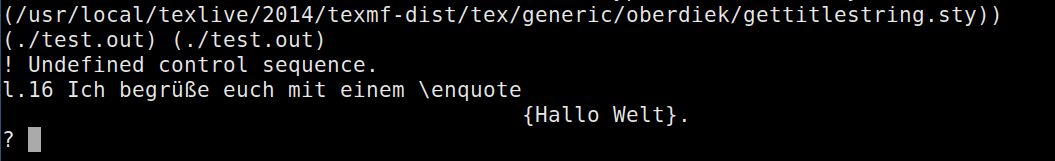
\includegraphics[width=0.9\textwidth]{figures/error1.png}
  \end{figure}
  \huge
  \begin{itemize}
    \item<2->[$\Rightarrow$] Vergessen \texttt{csquotes} zu laden.
  \end{itemize}
\end{frame}

\begin{frame}{Lösungsstrategien}
  \Large
  \begin{itemize}
    \item Angegebene Zeile und vorherige Zeilen kontrollieren
    \item Teile des Codes auskommentieren um Ort des Fehlers einzugrenzen
    \item \enquote{googlen}
    \item \href{tex.stackexchange.com}{tex.stackexchange.com}
  \end{itemize}
\end{frame}
